\chapter{Pha trộn, dao động, mômen lưỡng cực điện và toán tử trường}

Ta bắt đầu hơi lệch khỏi chủ đề đã thông báo, với một câu hỏi về neutrino. Có bằng chứng cho thấy neutrino có khối lượng và các loại neutrino pha trộn với nhau. Nếu khối lượng của chúng không hoàn toàn bằng nhau, làm thế nào một loại có thể biến đổi thành loại khác mà không vi phạm định luật bảo toàn năng lượng?

Câu hỏi này gợi ra một mô hình thường gặp trong cơ học lượng tử: trạng thái dùng để chuẩn bị hoặc phát hiện một hệ không nhất thiết là trạng thái chéo hóa Hamiltonian của hệ. Trạng thái có năng lượng xác định chỉ thu nhận một pha. Còn trạng thái được chuẩn bị dưới dạng chồng chập của nhiều mức năng lượng sẽ biến đổi vì các thành phần của nó thu nhận những pha khác nhau. Sự khác biệt ấy sẽ dẫn ta từ giếng thế đôi đến dao động neutrino và sự tiến động spin. Sau một đoạn xen kẽ về mômen lưỡng cực điện của electron, ta sẽ quay lại lượng tử hóa lần hai và thấy cùng cấu trúc Fourier vị trí--động lượng ở cấp độ toán tử.

\section{Vấn đề thực sự là sự pha trộn}

Neutrino không nhất thiết đều có cùng khối lượng. Các trạng thái riêng năng lượng không pha trộn với nhau; mỗi trạng thái tiến hóa độc lập. Điều ta gọi là \emph{loại} hay hương vị của neutrino gắn với cách nó được tạo ra và được phát hiện; một trạng thái hương vị có thể là tổ hợp tuyến tính của các trạng thái riêng năng lượng-khối lượng. Có thể biểu diễn sơ đồ như sau:
\begin{equation}
|\text{type}\rangle = \sum_n c_n |E_n\rangle .
\end{equation}
Vì vậy, phát biểu đúng không phải là các trạng thái riêng năng lượng biến đổi thành nhau, mà là những trạng thái được gọi là ``neutrino electron'' hoặc ``neutrino muon'' bản thân chúng không nhất thiết là trạng thái riêng năng lượng.

\begin{classroomqa}
\lecturetimestamp{00:00:09}
\audiencequestion{Nếu neutrino có khối lượng khác nhau, chúng có thể pha trộn như thế nào trong khi năng lượng vẫn được bảo toàn?}
\lecturerresponse{Các trạng thái riêng năng lượng-khối lượng không biến đổi thành nhau. Các trạng thái hương vị electron, muon và tau là những tổ hợp tuyến tính khác nhau của các trạng thái riêng ấy. Mỗi thành phần khối lượng tiến hóa với pha riêng của nó; sự giao thoa làm thay đổi xác suất hương vị mà không vi phạm định luật bảo toàn năng lượng.}
\end{classroomqa}

Có rất nhiều ví dụ về cấu trúc này. Ví dụ dễ thấy nhất bắt đầu với một hạt trong giếng thế đôi đối xứng.

\section{Giếng thế đôi đối xứng và các trạng thái định xứ gần đúng}

Xét một hạt chuyển động trong thế năng giếng đôi đối xứng, với một hàng rào cao ngăn cách hai cực tiểu. Nếu hàng rào cao vô hạn, hai giếng trái và phải sẽ hoàn toàn tách rời. Ta có thể giải bài toán cho giếng bên trái như thể giếng bên phải không tồn tại, và tương tự cho giếng bên phải. Khi đó, các hàm sóng trạng thái cơ bản gần đúng sẽ là trạng thái định xứ bên trái \(\psi_L\) và trạng thái định xứ bên phải \(\psi_R\), cả hai có cùng năng lượng \(E\).

Trong mỗi giếng cô lập, trạng thái cơ bản có những tính chất định tính quen thuộc: trơn, không có nút và có năng lượng thấp nhất có thể khi hạt bị giam giữ. Hãy hình dung hàng rào cao ở giữa như một bức tường gạch. Coi hàng rào là vô hạn chỉ là một phép gần đúng, nhưng phép gần đúng này cho ta một cặp trạng thái định xứ hữu ích để bắt đầu.

\begin{figure}
\centering
\begin{adjustbox}{max width=\linewidth}
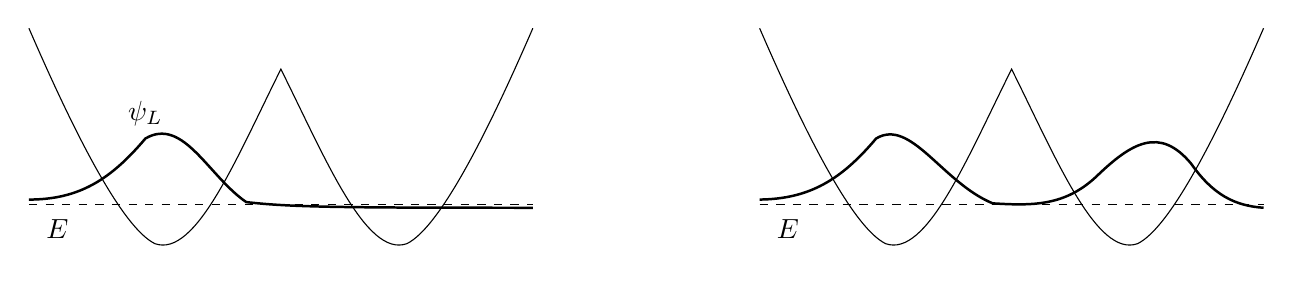
\begin{tikzpicture}[x=0.8cm,y=0.8cm]
\begin{scope}[shift={(-5.8,0)}]
\draw (-4,2.7) .. controls (-3.35,1.2) and (-2.55,-0.45) .. (-2.0,-0.72)
      .. controls (-1.35,-0.95) and (-0.7,0.65) .. (0,2.05)
      .. controls (0.7,0.65) and (1.35,-0.95) .. (2.0,-0.72)
      .. controls (2.55,-0.45) and (3.35,1.2) .. (4,2.7);
\draw[dashed] (-4,-0.10) -- (4,-0.10);
\node at (-3.55,-0.48) {$E$};
\draw[line width=0.9pt] (-4,-0.02) .. controls (-3.2,-0.02) and (-2.7,0.30) .. (-2.15,0.95)
      .. controls (-1.55,1.30) and (-1.15,0.35) .. (-0.55,-0.06)
      .. controls (0.15,-0.14) and (0.9,-0.15) .. (4,-0.15);
\node at (-2.15,1.35) {$\psi_L$};
\end{scope}
\begin{scope}[shift={(5.8,0)}]
\draw (-4,2.7) .. controls (-3.35,1.2) and (-2.55,-0.45) .. (-2.0,-0.72)
      .. controls (-1.35,-0.95) and (-0.7,0.65) .. (0,2.05)
      .. controls (0.7,0.65) and (1.35,-0.95) .. (2.0,-0.72)
      .. controls (2.55,-0.45) and (3.35,1.2) .. (4,2.7);
\draw[dashed] (-4,-0.10) -- (4,-0.10);
\node at (-3.55,-0.48) {$E$};
\draw[line width=0.9pt] (-4,-0.02) .. controls (-3.2,-0.01) and (-2.7,0.30) .. (-2.15,0.95)
      .. controls (-1.6,1.28) and (-1.1,0.25) .. (-0.30,-0.08)
      .. controls (0.35,-0.12) and (0.85,-0.12) .. (1.35,0.35)
      .. controls (1.9,0.88) and (2.35,1.15) .. (2.85,0.55)
      .. controls (3.2,0.05) and (3.55,-0.12) .. (4,-0.15);
\end{scope}
\end{tikzpicture}
\end{adjustbox}
\caption{Bản vẽ lại rõ nét các phác họa đầu tiên trên bảng. Hình bên trái là trạng thái thử chỉ nằm ở một phía \(\psi_L\), thu được bằng cách giả sử hàng rào hiệu dụng là vô hạn. Ở hình bên phải, cùng hàm sóng được kéo dài đối xứng qua hàng rào, minh họa sự rò qua hàng rào tuy nhỏ nhưng khác không; chính sự rò này cuối cùng tạo nên trạng thái cơ bản chẵn thực sự.}
\end{figure}

Tuy nhiên, trong cơ học lượng tử, hàng rào không thực sự vô hạn. Hàm sóng trong vùng hàng rào không chính xác bằng không; nó chỉ rất nhỏ. Sự rò rất nhỏ này chính là mấu chốt. Nó biến mô tả gần đúng trái-phải thành một bài toán pha trộn thực sự.

\section{Các trạng thái riêng parity và độ tách mức hàm mũ}

Mô tả định xứ giờ đây bị ngắt quãng bởi một định lý: nếu thế năng đối xứng, các hàm riêng năng lượng chính xác có thể được chọn sao cho chúng đối xứng hoặc phản đối xứng qua phép phản xạ.

\begin{theorem}
Nếu \(V(x)=V(-x)\) trong một chiều, thì có thể chọn các hàm riêng của Hamiltonian thỏa mãn một trong hai điều kiện
\[
\psi(x)=\psi(-x)
\qquad \text{or} \qquad
\psi(x)=-\psi(-x).
\]
\end{theorem}

Giờ là phần hiệu chỉnh. Các trạng thái một phía \(\psi_L\) và \(\psi_R\) không đối xứng cũng không phản đối xứng, nên chúng không thể là trạng thái riêng chính xác của Hamiltonian đầy đủ. Chúng chỉ là các trạng thái gần đúng tốt khi hàng rào cao. Các trạng thái riêng thực sự là những tổ hợp đối xứng và phản đối xứng,
\begin{align}
\psi_+ &= \frac{\psi_L+\psi_R}{\sqrt{2}},\\
\psi_- &= \frac{\psi_L-\psi_R}{\sqrt{2}}.
\end{align}
Dùng ký hiệu sẽ giữ nguyên trên bảng, ta ký hiệu năng lượng của chúng là
\begin{align}
H\psi_+ &= (E_1-\epsilon)\psi_+,\\
H\psi_- &= (E_1+\epsilon)\psi_-.
\end{align}
Do đó, độ tách mức tổng cộng là
\begin{equation}
\Delta E = (E_1+\epsilon)-(E_1-\epsilon)=2\epsilon .
\end{equation}

\begin{figure}[htbp]
\centering
\includegraphics[width=0.92\linewidth]{lecture_08_frame_02.png}
\caption{Hàm sóng được kéo dài đối xứng trong thế giếng đôi. Biên độ dưới hàng rào nhỏ nhưng khác không; đây là nguồn gốc của độ tách mức.}
\lectureframe{00:06:19}
\end{figure}

\begin{figure}
\centering
\begin{tikzpicture}[x=1cm,y=1cm]
\draw[->] (0,0) -- (0,3);
\node[left] at (0,2.8) {energy};
\draw (-0.35,1.60) -- (0.35,1.60);
\node[left] at (-0.45,1.60) {$\psi_L,\psi_R$};
\node at (1.7,1.60) {$\Longrightarrow$};
\draw (3.0,1.32) -- (3.75,1.32);
\draw (3.0,1.88) -- (3.75,1.88);
\draw[dashed] (2.8,1.60) -- (3.95,1.60);
\node[right] at (3.9,1.32) {$\psi_+,\ E_1-\epsilon$};
\node[right] at (3.9,1.88) {$\psi_-,\ E_1+\epsilon$};
\node[below] at (3.37,1.60) {$E_1$};
\end{tikzpicture}
\caption{Lập luận trên bảng về độ tách mức do xuyên hầm. Các trạng thái trái và phải gần đúng gần suy biến, nhưng các trạng thái riêng chẵn và lẻ chính xác bị tách nhau một lượng nhỏ \(2\epsilon\).}
\end{figure}

Thứ tự các mức thể hiện điểm cốt yếu về mặt vật lý. Trạng thái đối xứng có năng lượng thấp hơn một chút vì nó trơn hơn trong vùng hàng rào; cho phép hàm sóng rò qua và tiếp tục đối xứng làm giảm năng lượng một lượng rất nhỏ. Trạng thái phản đối xứng có năng lượng cao hơn một chút vì trạng thái kích thích thứ nhất trong một chiều có một nút, và trong bài toán đối xứng này nút nằm ở trung điểm. Độ cong tăng thêm làm tăng động năng.

Hiệu ứng này rất nhỏ, nhỏ theo hàm mũ của chiều rộng và chiều cao hàng rào. Ở đây ta không cần công thức WKB tường minh; điều quan trọng là độ tách mức có thật nhưng rất nhỏ. Cũng cần nhớ rằng dấu tổng thể của hàm sóng không mang thông tin vật lý. Thay \(\psi_-\) bằng \(-\psi_-\) không làm thay đổi trạng thái.

\section{Sự tiến hóa theo thời gian và dao động trái-phải}

Giờ hãy đặt câu hỏi về động lực học: điều gì xảy ra nếu ta đặt một hạt vào giếng bên trái? Đây là bước quyết định, vì dao động là biểu hiện phụ thuộc thời gian của chính hiện tượng pha trộn ấy.

Các hệ thức ngược là
\begin{align}
\psi_L &= \frac{\psi_+ + \psi_-}{\sqrt{2}},\\
\psi_R &= \frac{\psi_+ - \psi_-}{\sqrt{2}}.
\end{align}
Vậy trạng thái ban đầu định xứ bên trái là
\begin{equation}
\psi(0)=\psi_L=\frac{\psi_+ + \psi_-}{\sqrt{2}}.
\end{equation}
Đây không phải trạng thái riêng năng lượng, nên nó phải tiến hóa một cách không tầm thường.

Ta dùng quy ước Schr\"odinger chuẩn \(e^{-iEt}\). Một pha chung không gây ra hiệu ứng quan sát được; chỉ có pha tương đối giữa hai thành phần năng lượng mới có thể chuyển xác suất từ giếng này sang giếng kia.

Theo quy ước đó,
\begin{equation}
\psi(t)=\frac{1}{\sqrt{2}}\left(e^{-i(E_1-\epsilon)t}\psi_+ + e^{-i(E_1+\epsilon)t}\psi_-\right).
\end{equation}
Đây là phiên bản đã chỉnh lý của công thức trên bảng. Bây giờ ta đặt pha chung ra ngoài:
\begin{equation}
\psi(t)=\frac{e^{-iE_1 t}}{\sqrt{2}}\left(e^{i\epsilon t}\psi_+ + e^{-i\epsilon t}\psi_-\right).
\end{equation}
Một pha giờ quay theo một chiều quanh đường tròn đơn vị, pha kia quay theo chiều ngược lại. Trạng thái chỉ thay đổi vì hai pha này lệch nhịp với nhau.

Để thấy rõ dao động trái-phải, thay các định nghĩa của \(\psi_\pm\) vào biểu thức:
\begin{align}
\psi(t)
&= \frac{e^{-iE_1 t}}{2}
\left[e^{i\epsilon t}(\psi_L+\psi_R)+e^{-i\epsilon t}(\psi_L-\psi_R)\right] \\
&= \frac{e^{-iE_1 t}}{2}
\left[(e^{i\epsilon t}+e^{-i\epsilon t})\psi_L+(e^{i\epsilon t}-e^{-i\epsilon t})\psi_R\right] \\
&= e^{-iE_1 t}\left[\psi_L\cos(\epsilon t)+i\,\psi_R\sin(\epsilon t)\right].
\end{align}
Đây là phần suy diễn có lời giải then chốt của chương. Trong phép gần đúng hai trạng thái, với \(\psi_L\) và \(\psi_R\) trực chuẩn, xác suất là
\begin{equation}
P_L(t)=\cos^2(\epsilon t),
\qquad
P_R(t)=\sin^2(\epsilon t).
\end{equation}
Vì vậy, hệ dao động. Ở những thời điểm trung gian, trạng thái thực sự là một chồng chập; chẳng hạn, khi \(\epsilon t=\pi/4\), xác suất ở hai phía bằng nhau. Các pha tiến hóa liên tục, và trạng thái định xứ cũng thay đổi liên tục theo chúng.

Phần suy diễn trên bảng xác định thời điểm đầu tiên mà dấu tương đối đổi chiều. Ta tìm thời điểm sao cho
\begin{equation}
e^{-i\epsilon t}=-\,e^{i\epsilon t},
\end{equation}
đây là mốc dễ thấy trên bảng. Nhân hai vế ta được
\begin{equation}
e^{2i\epsilon t}=-1.
\end{equation}
Ở lần đầu tiên điều này xảy ra,
\begin{equation}
2\epsilon t=\pi,
\qquad\text{so}\qquad
t_{L\to R}=\frac{\pi}{2\epsilon}.
\end{equation}

\begin{figure}[htbp]
\centering
\includegraphics[width=0.94\linewidth]{lecture_08_frame_05.png}
\caption{Tính toán pha tương đối trên bảng. Hai thành phần năng lượng trở nên ngược pha khi \(e^{2i\epsilon t}=-1\), cho thời gian chuyển trạng thái lần đầu \(2\epsilon t=\pi\). Phần suy diễn được trình bày bằng chữ dùng nhất quán quy ước pha Schr\"odinger.}
\lectureframe{00:17:52}
\end{figure}
Tại thời điểm đó,
\begin{equation}
\psi(t_{L\to R}) \propto \frac{\psi_+-\psi_-}{\sqrt{2}}=\psi_R.
\end{equation}
Pha tổng thể không quan trọng. Điều cốt yếu là hạt ban đầu được đặt ở bên trái đã tiến hóa thành trạng thái định xứ bên phải. Sau một khoảng thời gian bằng như vậy nữa, nó lại dao động trở về. Pha trộn và dao động luôn đi cùng nhau.

Phương trình rất rõ ràng: \(\epsilon\) nhỏ thì dao động chậm và thời gian chuyển trạng thái dài. Không trạng thái định xứ nào có năng lượng xác định, nhưng hai thành phần năng lượng chính xác vẫn bảo toàn năng lượng và tiến hóa đúng như dự kiến.

\section{Các phép tương tự với neutrino, amoniac và spin}

Giếng đôi cung cấp cho ta khuôn mẫu để hiểu câu hỏi ban đầu về neutrino. Neutrino được tạo ra cùng với một electron được gọi là neutrino electron; neutrino được tạo ra cùng với một muon được gọi là neutrino muon. Các nhãn hương vị này mô tả các kênh tạo ra và phát hiện neutrino. Một cơ sở khác gồm các trạng thái có khối lượng xác định, và do đó có năng lượng hạt tự do xác định khi động lượng cố định.

Trong mô hình minh họa đơn giản nhất gồm hai trạng thái pha trộn cực đại,
\begin{equation}
|\nu_e\rangle \sim \frac{|m_1\rangle+|m_2\rangle}{\sqrt{2}},
\qquad
|\nu_\mu\rangle \sim \frac{|m_1\rangle-|m_2\rangle}{\sqrt{2}},
\end{equation}
trong đó các trạng thái riêng khối lượng đóng vai trò của \(\psi_+\) và \(\psi_-\), còn các trạng thái hương vị đóng vai trò của \(\psi_L\) và \(\psi_R\). Sự pha trộn neutrino thực tế dùng một ma trận pha trộn không tầm thường thay cho các hệ số bằng nhau này, nhưng cơ chế đã thể hiện rõ ở đây.

Neutrino electron được tạo ra trong một quá trình có electron tham gia, cũng như một hạt có thể được đặt vào giếng bên trái. Trong một quãng đường ngắn, hai thành phần khối lượng của nó tích lũy các pha gần như bằng nhau, nên khi tương tác, nó vẫn được nhận diện là có hương vị electron. Sau khi truyền đi một quãng đường dài, các pha của chúng tách biệt. Khi đó, tương tác dòng tích điện về sau có thể tạo ra muon thay vì electron: trạng thái đã có thêm thành phần hương vị muon. Lặp lại thí nghiệm ở các khoảng cách hoặc năng lượng khác nhau sẽ cho thấy dao động.

Điều này không mâu thuẫn với định luật bảo toàn năng lượng. Các trạng thái riêng năng lượng-khối lượng làm đúng như những gì được kỳ vọng ở trạng thái riêng. Chính chồng chập hương vị mới tiến hóa. Trong giới hạn tương đối tính, pha tương đối quan sát được phụ thuộc vào hiệu bình phương khối lượng, có dạng sơ đồ như sau
\begin{equation}
\Delta\phi_{ij}\simeq \frac{\Delta m_{ij}^{,2}L}{2E}.
\end{equation}
Do đó, dao động cho thấy không phải mọi khối lượng neutrino đều giống hệt nhau; ít nhất hai trạng thái riêng khối lượng có khối lượng khác nhau.

\begin{classroomqa}
\lecturetimestamp{00:24:06}
\audiencequestion{Điều gì quyết định độ tách nhỏ \(\epsilon\) trong ví dụ giếng đôi?}
\lecturerresponse{Độ tách này phụ thuộc vào khối lượng hạt, cũng như chiều cao và chiều rộng của hàng rào. Xuyên hầm phụ thuộc theo hàm mũ vào những đặc điểm ấy, nên chỉ cần thay đổi hàng rào vừa phải cũng có thể làm thay đổi lớn theo tỷ lệ của \(\epsilon\).}
\end{classroomqa}

\begin{classroomqa}
\lecturetimestamp{00:24:26}
\audiencequestion{Hiện tượng dao động này đã thực sự được quan sát chưa?}
\lecturerresponse{Có. Độ tách mức do xuyên hầm được quan sát trong các hệ lượng tử thông thường, còn dao động hương vị được quan sát ở neutrino. Cơ chế vi mô khác nhau, nhưng cả hai đều thể hiện cùng kiểu tiến hóa pha của hệ hai trạng thái.}
\end{classroomqa}

\begin{classroomqa}
\lecturetimestamp{00:24:34}
\audiencequestion{Dao động neutrino liên hệ thế nào với khối lượng neutrino?}
\lecturerresponse{Các trạng thái riêng truyền đi có khối lượng khác nhau nên tích lũy các pha khác nhau. Sự giao thoa giữa chúng làm thay đổi thành phần hương vị. Trong mô tả tương đối tính thực tế, hiệu bình phương khối lượng mới chi phối dao động, chứ không phải khối lượng của một hạt biến thiên theo thời gian theo nghĩa đen.}
\end{classroomqa}

\begin{classroomqa}
\lecturetimestamp{00:25:02}
\audiencequestion{Khối lượng neutrino chỉ là lý thuyết đang chiếm ưu thế, hay là sự thật thực nghiệm?}
\lecturerresponse{Dao động là sự thật thực nghiệm và đòi hỏi các hiệu khối lượng khác không. Thang khối lượng tuyệt đối là một đại lượng riêng biệt và khó đo hơn, nhưng bức tranh tối giản trong đó mọi neutrino đều không có khối lượng đã bị thực nghiệm bác bỏ.}
\end{classroomqa}

\subsection{Sự nghịch đảo của amoniac: một hàng rào theo nghĩa đen}

Phân tử amoniac, \(\mathrm{NH}_3\), có dạng chóp tam giác: ba nguyên tử hydro nằm trên một mặt phẳng, còn nitơ ở một phía của mặt phẳng đó. Có một cấu hình tương đương trong đó nitơ ở phía bên kia. Hai cấu hình định xứ này không phải các trạng thái dừng chính xác. Nitơ có thể xuyên hầm qua mặt phẳng hydro, tạo ra các trạng thái riêng năng lượng đối xứng và phản đối xứng, cùng độ tách mức nghịch đảo nhỏ. Đây là nguồn gốc vật lý của chính toán học ấy trong maser amoniac.

\begin{classroomqa}
\lecturetimestamp{00:25:11}
\audiencequestion{Trong amoniac, hàng rào có phải là cấu hình trong đó nitơ đi qua mặt phẳng hydro không?}
\lecturerresponse{Đúng. Năng lượng phân tử đạt cực tiểu ở mỗi cấu hình dạng chóp, còn cấu hình phẳng có năng lượng cao hơn. Xuyên hầm qua cấu hình đó ghép nối hai phía.}
\end{classroomqa}

\begin{classroomqa}
\lecturetimestamp{00:27:10}
\audiencequestion{Hàng rào vật lý tương ứng giữa neutrino electron và neutrino muon là gì?}
\lecturerresponse{Không có hàng rào không gian theo nghĩa đen. Phép tương tự ở đây là về mặt đại số: một tương tác ngoài đường chéo trong Hamiltonian neutrino làm pha trộn cơ sở hương vị. Trong amoniac, tương tác đó bắt nguồn từ xuyên hầm; với neutrino, nó là một phần của cấu trúc khối lượng và pha trộn.}
\end{classroomqa}

\subsection{Sự tiến động spin: pha trộn không cần xuyên hầm}

Ta đã gặp cùng một cấu trúc đại số ở spin. Xét hai trạng thái \(|\uparrow_z\rangle\) và \(|\downarrow_z\rangle\). Khi không có từ trường, chúng suy biến. Bây giờ bật từ trường theo hướng \(x\). Các trạng thái riêng năng lượng không còn là các trạng thái riêng \(z\), mà là các trạng thái phân cực theo \(x\). Dùng tạm các tên trái--phải trên bảng,
\begin{align}
|L_x\rangle &= \frac{|\uparrow_z\rangle+|\downarrow_z\rangle}{\sqrt{2}},\\
|R_x\rangle &= \frac{|\uparrow_z\rangle-|\downarrow_z\rangle}{\sqrt{2}}.
\end{align}
Đây là các trạng thái tương tự trực tiếp với \(\psi_+\) và \(\psi_-\). Mômen từ song song và đối song song với từ trường có năng lượng hơi khác nhau. Nếu các năng lượng ấy là \(E\mp\epsilon\), thì spin ban đầu hướng lên tiến hóa như sau
\begin{equation}
|\uparrow_z,t\rangle
= e^{-iEt}\left[\cos(\epsilon t)\,|\uparrow_z\rangle
+ i\sin(\epsilon t)\,|\downarrow_z\rangle\right].
\end{equation}
Đây là cùng công thức như với giếng đôi, chỉ khác là giờ đây sự tiến hóa liên tục là sự tiến động spin quanh trục \(x\). Bắt đầu từ \(+z\), spin đi qua các hướng ngang, đạt \(-z\) sau nửa chu kỳ tiến động, rồi trở lại sau nửa chu kỳ nữa. Phép đo \(S_z\) vẫn chỉ cho kết quả lên hoặc xuống; trạng thái spin biến thiên liên tục quyết định xác suất thu được mỗi kết quả. Cơ chế này không cần xuyên hầm. Điều kiện duy nhất là Hamiltonian phải chéo trong một cơ sở khác với cơ sở dùng để chuẩn bị trạng thái.

\begin{classroomqa}
\lecturetimestamp{00:32:25}
\audiencequestion{Trong bức tranh này, neutrino tau ra sao?}
\lecturerresponse{Nó cũng pha trộn. Bài toán thực có ba trạng thái hương vị và ba trạng thái khối lượng, nên một ma trận pha trộn ba nhân ba thay cho phép quay hai trạng thái. Nguyên lý giao thoa pha vẫn không đổi.}
\end{classroomqa}

\begin{classroomqa}
\lecturetimestamp{00:32:57}
\audiencequestion{Ngay sau khi áp dụng từ trường ngang, spin vẫn hướng lên chứ, và nó có thể hướng về phía chúng ta hoặc ra xa chúng ta không?}
\lecturerresponse{Trong khoảng thời gian rất ngắn, gần như chắc chắn spin vẫn hướng lên, với xác suất hướng xuống nhỏ. Trạng thái tiến động liên tục quanh trục từ trường và đi qua các hướng ngang \(\pm y\), đồng thời vẫn vuông góc với từ trường hướng theo \(x\) nếu ban đầu nó vuông góc với từ trường. Phép đo theo bất kỳ trục tùy chọn nào vẫn cho một trong các trị riêng rời rạc của trục đó.}
\end{classroomqa}

\begin{classroomqa}
\lecturetimestamp{00:34:30}
\audiencequestion{Có phải ta chọn từ trường yếu để spin không bao giờ hướng dọc theo từ trường không?}
\lecturerresponse{Không. Hình học của chuyển động là hệ quả của sự tiến động quanh trục từ trường, chứ không phải do từ trường yếu. Từ trường yếu chỉ làm độ tách năng lượng và tần số tiến động nhỏ đi, khiến dao động chậm, tương tự ví dụ neutrino.}
\end{classroomqa}

Độ mạnh pha trộn neutrino và khối lượng nhỏ của neutrino là những tham số mà Mô hình Chuẩn tối giản theo cách xây dựng ban đầu không giải thích được nguồn gốc sâu xa. Vì thế, khối lượng neutrino cho thấy vật lý vượt ra ngoài mô hình tối giản ấy, dù thang đo quan sát được rất nhỏ và có thể phản ánh vật lý ở một thang năng lượng rất xa.

\begin{classroomqa}
\lecturetimestamp{00:36:27}
\audiencequestion{Có phải nhờ hiện tượng dao động mà ta biết neutrino có khối lượng không?}
\lecturerresponse{Đây là bằng chứng trực tiếp có tính quyết định cho thấy các thành phần truyền đi có khối lượng khác nhau. Nếu mọi thành phần liên quan đều chính xác không có khối lượng và suy biến, chúng sẽ không tích lũy pha tương đối phụ thuộc khối lượng, và sẽ không có kiểu dao động hương vị trong chân không này.}
\end{classroomqa}

\begin{classroomqa}
\lecturetimestamp{00:37:57}
\audiencequestion{Sau nửa chu kỳ, neutrino có nên biểu hiện một nửa như hương vị electron và một nửa như hương vị muon không?}
\lecturerresponse{Trong mô hình lý tưởng đối xứng hai trạng thái, xác suất bằng nhau xuất hiện tại một phần tư chu kỳ xác suất đầy đủ, còn sự chuyển đổi hoàn toàn xảy ra tại cực đại đầu tiên. Dao động ba hương vị thực có các góc pha trộn không bằng nhau, nhiều tần số, các ràng buộc spin-độ xoắn và hiệu ứng vật chất, nên sự chuyển đổi đối xứng hoàn toàn không phải là trường hợp tổng quát.}
\end{classroomqa}

\begin{classroomqa}
\lecturetimestamp{00:38:36}
\audiencequestion{Nếu các thành phần khối lượng khác nhau, vận tốc của neutrino Mặt Trời có nhất thiết phải thay đổi để bảo toàn động lượng không?}
\lecturerresponse{Trạng thái hương vị là chồng chập kết hợp của các thành phần có khối lượng cố định; khối lượng của nó không phải một đại lượng cổ điển dao động theo thời gian. Trong mô tả thường dùng với động lượng bằng nhau, các thành phần có năng lượng và vận tốc nhóm hơi khác nhau; còn trong mô tả năng lượng bằng nhau, chúng có động lượng hơi khác nhau. Nếu được xử lý nhất quán, cả hai quy ước đều cho cùng pha dao động quan sát được.}
\end{classroomqa}

Sự tiến hóa pha này đã giải quyết sự thiếu hụt neutrino Mặt Trời từng được phát hiện trước đây. Các máy dò đời đầu chủ yếu nhạy với neutrino electron, nên neutrino rời Mặt Trời dưới dạng hương vị electron có thể đến nơi một phần mang hương vị muon hoặc tau và không được ghi nhận qua kênh đó. Tính toán chi tiết về Mặt Trời bao gồm sự pha trộn ba hương vị và hiệu ứng vật chất, nhưng bài học khái niệm đã có trong giếng đôi: việc chuẩn bị và sự truyền đi sử dụng các cơ sở khác nhau.

\section{Đoạn xen kẽ: mômen lưỡng cực điện, tính đối xứng và khẳng định ``“Hình cầu electron”''}

Vì ta đang bàn về hiện tượng học hạt, hãy tạm rời toán học hình thức. Một bài viết đại chúng mô tả giới hạn mới về mômen lưỡng cực điện của electron bằng cách nói rằng electron đã được chứng minh là hình cầu. Khẩu hiệu ấy nhập nhằng ba câu hỏi khác nhau: mômen lưỡng cực điện đo đại lượng gì, tính đối xứng quay có nghĩa gì đối với một trạng thái lượng tử, và thí nghiệm thực sự đã đặt ra giới hạn nào.

\subsection{Đại lượng nào đã được đo?}

Đại lượng được đo, hay đúng hơn là được đặt giới hạn, là mômen lưỡng cực điện của electron. Với các điện tích tách rời \(\pm q\), mômen lưỡng cực là
\begin{equation}
\mathbf d = q\,\boldsymbol{\ell},
\end{equation}
trong đó \(\boldsymbol{\ell}\) là vectơ phân cách. Mômen lưỡng cực khác không có nghĩa là phân bố điện tích bị lệch so với một tâm nào đó.

Tuy nhiên, với electron, câu hỏi thích hợp không chỉ là điện tích có lệch tâm theo một hướng tùy ý nào đó hay không. Electron có spin, do đó có một trục. Nó cũng có mômen từ. Câu hỏi có ý nghĩa vật lý là liệu có tương quan giữa độ lệch của điện tích và trục ấy hay không:
\begin{equation}
\mathbf d_e \parallel \boldsymbol{\mu}_e
\qquad \text{or equivalently} \qquad
\mathbf d_e \parallel \mathbf S .
\end{equation}
Đó chính là điều được gọi là mômen lưỡng cực điện của electron. Về mặt khái niệm, ta xét xem đặt một electron phân cực spin trong điện trường có làm tách hai định hướng spin hay không:
\begin{equation}
H_{\mathrm{EDM}}=-\mathbf d_e\cdot \mathbf E,
\qquad
\mathbf d_e=d_e\frac{\mathbf S}{|\mathbf S|}.
\end{equation}
Thí nghiệm thực tế trên bàn thí nghiệm tinh vi hơn nhiều so với hình dung một electron trần nằm giữa hai bản tụ điện, nhưng đây là ý tưởng về tính đối xứng và độ dịch chuyển năng lượng mà thí nghiệm khai thác.

\subsection{Vì sao không có mômen lưỡng cực điện không đồng nghĩa với hình cầu}

Điều chỉnh đầu tiên rất cơ bản. Một vật có thể không có mômen lưỡng cực mà vẫn không có dạng cầu. Một ellipsoid có tâm trùng với tâm điện tích có lượng điện tích ở mỗi phía bằng nhau nên không có lưỡng cực, nhưng vẫn có thể có mômen tứ cực. Một phân bố phức tạp hơn nữa có thể không có mômen lưỡng cực cũng không có mômen tứ cực, nhưng vẫn có mômen đa cực bậc cao hơn. Đo một hệ số đa cực không thể xác định toàn bộ hình dạng.

Trong cơ học lượng tử, từ ``hình dạng'' trở nên tinh tế hơn. Hãy hình dung một phân tử giống quả tạ gồm hai nguyên tử, với độ dài liên kết gần như cố định. Bỏ qua dao động xuyên tâm và chỉ xét chuyển động quay. Các trạng thái quay được xác định bởi mômen động lượng. Nếu phân tử là boson, trạng thái quay thấp nhất có \(J=0\). Vì mômen động lượng sinh ra phép quay,
\begin{equation}
\begin{gathered}
J=0 \quad\Longrightarrow\\
\text{rotationally invariant ground state.}
\end{gathered}
\end{equation}
trạng thái lượng tử bất biến qua phép quay, dù mọi hình dung theo một định hướng xác định đều trông như quả tạ. Có thể mô tả trạng thái này là chồng chập kết hợp của mọi định hướng. Gọi trạng thái là ``hình cầu'' hữu ích đối với một số phép đo nhưng có thể gây hiểu lầm đối với những phép đo khác.

Hãy chụp nhanh một ảnh. Chụp nhanh ở đây là phép đo định hướng; phép đo định hướng đủ chính xác đưa hệ vào trạng thái định xứ theo góc. Trạng thái như vậy không thể đồng thời có mômen động lượng xác định. Đây là dạng quay của nguyên lý bất định vị trí--động lượng: định xứ góc tất yếu làm xuất hiện độ trải của mômen động lượng, do đó kích thích chuyển động quay.

Với một vật quay cứng,
\begin{equation}
E_J=\frac{J(J+1)}{2I},
\end{equation}
như vậy năng lượng cần để phân giải cấu trúc phụ thuộc vào mômen quán tính \(I\). Một quả tạ dùng trong phòng tập có \(I\) rất lớn và các mức quay cách nhau cực kỳ sít; ánh sáng thông thường có thể dễ dàng làm nhiễu nó đủ để bộc lộ một định hướng. Các mức của phân tử cách nhau xa hơn. Các mức của hadron gọn đặc còn cách xa hơn nhiều. Nếu đầu dò không đủ năng lượng để kích thích cấu trúc quay đầu tiên có thể phân giải, các phép đo lặp lại chỉ thấy trạng thái cơ bản đã lấy trung bình theo phép quay.

Có thể hình dung meson một cách sơ lược như một hệ hai hạt gồm quark--phản quark. Các kích thích quỹ đạo đầu tiên cần năng lượng hàng trăm triệu electron vôn hoặc hơn, cao hơn rất nhiều so với năng lượng của photon quang học. Vì thế, đầu dò năng lượng thấp không thể chụp nhanh để thấy định hướng bên trong. ``Có hình cầu hay không'' một phần phụ thuộc vào trạng thái được chuẩn bị và một phần vào độ phân giải của thiết bị.

Electron làm vấn đề này rõ hơn. Đây là hạt có spin-\(\tfrac12\), chứ không phải một đại lượng vô hướng quay. Trạng thái phân cực spin mang một trục và một mômen từ. Hình dung quen thuộc về điện tích quay quanh trục ấy chỉ là một cách diễn giải gợi hình---hạt Dirac dạng điểm không thực sự là một quả cầu nhỏ đang quay---nhưng cách hình dung này nhắc đúng rằng mômen từ đổi chiều khi spin đổi chiều. Câu hỏi về mômen lưỡng cực điện là liệu độ lệch của điện tích có tương quan với chính trục ấy hay không. Kết quả bằng không không biến electron thành một quả cầu cổ điển.

\begin{classroomqa}
\lecturetimestamp{00:57:30}
\audiencequestion{Nếu một phần điện tích của electron bị dịch chuyển, điều đó có vi phạm tính lượng tử hóa điện tích không?}
\lecturerresponse{Không. Tính lượng tử hóa điện tích ấn định tổng điện tích. Mômen lưỡng cực liên quan đến mômen không gian bậc nhất của phân bố điện tích đó, hoặc tương đương là một tương tác được phép giữa hạt điểm với điện trường; nó không đòi hỏi tổng điện tích phải thay đổi một lượng phân số.}
\end{classroomqa}

\begin{classroomqa}
\lecturetimestamp{00:58:00}
\audiencequestion{Mômen lưỡng cực điện có bị lý thuyết trường lượng tử cấm không?}
\lecturerresponse{Bản thân lý thuyết trường lượng tử không cấm chúng. Chúng bị cấm khi một số đối xứng rời rạc nhất định là chính xác. Khi các đối xứng ấy bị vi phạm, toán tử mômen lưỡng cực điện được phép xuất hiện, dù hệ số của nó có thể cực kỳ nhỏ.}
\end{classroomqa}

\subsection{Tính chẵn lẻ và phép đảo ngược thời gian}

Nội dung thực sự của phần thảo luận về mômen lưỡng cực điện là tính đối xứng. Dưới phép biến đổi chẵn lẻ, mômen lưỡng cực điện biến đổi như một vectơ cực thông thường, còn mômen từ biến đổi như một vectơ trục:
\begin{align}
P:\qquad &\mathbf d_e \to -\mathbf d_e,
&\boldsymbol{\mu}_e \to \boldsymbol{\mu}_e .
\end{align}
Dưới phép đảo ngược thời gian, dòng điện tuần hoàn xác định mômen từ đổi chiều, còn độ lệch tĩnh của điện tích thì không:
\begin{align}
T:\qquad &\mathbf d_e \to \mathbf d_e,
&\boldsymbol{\mu}_e \to -\boldsymbol{\mu}_e .
\end{align}
Vì vậy, một mômen lưỡng cực điện khác không, song song với trục spin của electron, bị cấm nếu đối xứng chẵn lẻ là chính xác, và cũng bị cấm nếu đối xứng đảo ngược thời gian là chính xác:
\begin{equation}
(P\ \text{exact}) \Rightarrow \mathbf d_e=0,
\qquad
(T\ \text{exact}) \Rightarrow \mathbf d_e=0.
\end{equation}

Cần nói rõ hình học ở đây. Mômen từ được tạo ra bởi dòng điện chạy thành vòng. Phép phản xạ gương đảo chiều các vectơ cực thông thường, nhưng giữ nguyên vectơ trục vuông góc với vòng dây đó. Độ dời điện tích dọc theo trục thì đổi chiều. Vì vậy, electron có \(\mathbf d_e\) song song với \(\boldsymbol\mu_e\) sẽ bị phản xạ thành electron có cùng chiều mômen từ nhưng quan hệ giữa mômen điện và mômen từ thì ngược lại. Nếu đối xứng chẵn lẻ là chính xác và chỉ có một loại electron, thì hai mô tả này phải biểu diễn cùng một hạt; chỉ \(d_e=0\) là phù hợp.

Phép đảo ngược thời gian dẫn đến cùng kết luận theo một cách khác. Chiếu cuộn phim ngược chiều thời gian làm dòng điện đổi chiều, do đó \(\boldsymbol\mu_e\) cũng đổi chiều, nhưng không làm độ dời điện tích tĩnh chuyển động. Một trạng thái có hai mômen song song biến thành trạng thái có hai mômen ngược chiều. Đối xứng đảo ngược thời gian chính xác cũng sẽ đòi hỏi \(d_e=0\).

\begin{figure}[htbp]\centering
\begin{tikzpicture}[>=Stealth,scale=0.95]
  \node[font=\bfseries] at (1.0,2.25) {original};
  \draw[->,very thick,blue!70!black] (0.65,0) -- (0.65,1.65);
  \draw[->,very thick,red!75!black] (1.35,0) -- (1.35,1.65);
  \node[blue!70!black,below] at (0.65,0) {$\boldsymbol\mu$};
  \node[red!75!black,below] at (1.35,0) {$\mathbf d$};

  \node[font=\bfseries] at (4.5,2.25) {parity};
  \draw[->,very thick,blue!70!black] (4.15,0) -- (4.15,1.65);
  \draw[->,very thick,red!75!black] (4.85,1.65) -- (4.85,0);
  \node[blue!70!black,below] at (4.15,0) {$\boldsymbol\mu$};
  \node[red!75!black,below] at (4.85,0) {$-\mathbf d$};

  \node[font=\bfseries] at (8.0,2.25) {time reversal};
  \draw[->,very thick,blue!70!black] (7.65,1.65) -- (7.65,0);
  \draw[->,very thick,red!75!black] (8.35,0) -- (8.35,1.65);
  \node[blue!70!black,below] at (7.65,0) {$-\boldsymbol\mu$};
  \node[red!75!black,below] at (8.35,0) {$\mathbf d$};
\end{tikzpicture}\caption{Phép kiểm tra đối xứng được dựng lại từ lập luận trên bảng. Phép biến đổi chẵn lẻ đảo chiều mômen lưỡng cực điện nhưng không đảo chiều mômen từ dạng vectơ trục; phép đảo ngược thời gian đảo chiều mômen từ nhưng không đảo chiều độ dời điện tích tĩnh. Nếu một trong hai đối xứng là chính xác, mômen lưỡng cực điện vĩnh cửu song song với spin sẽ bị cấm.}\end{figure}

\begin{figure}[htbp]\centering
\includegraphics[width=0.94\linewidth]{lecture_08_frame_06.png}\caption{Các hình phác họa trục từ và độ dời điện tích đặt cạnh nhau trong phần lập luận về phép đảo ngược thời gian. Sơ đồ TikZ gọn ở trên tách riêng nội dung của phép biến đổi khỏi phần bảng trực tiếp đã bị xóa một phần.}\lectureframe{01:06:10}\end{figure}

\begin{classroomqa}\lecturetimestamp{01:06:38}\audiencequestion{Khi đảo ngược thời gian, cả dòng điện lẫn điện tích có đổi chiều không?}\lecturerresponse{Dòng điện đổi chiều vì vận tốc đổi chiều; bản thân điện tích thì không. Phép liên hợp điện tích \(C\), chứ không phải phép đảo ngược thời gian \(T\), làm điện tích đổi dấu.}\end{classroomqa}

\begin{classroomqa}\lecturetimestamp{01:07:01}\audiencequestion{Tính phản đơn nhất của phép đảo ngược thời gian có nghĩa là cơ học lượng tử phi tương đối tính không bất biến dưới phép đảo ngược thời gian không?}\lecturerresponse{Không. Tính phản đơn nhất chính là cách biểu diễn nhất quán phép đảo ngược thời gian trong cơ học lượng tử: phép này lấy liên hợp phức các biên độ và đảo chiều động lượng cùng spin. Một Hamiltonian cụ thể có bất biến hay không là câu hỏi riêng.}\end{classroomqa}

\begin{classroomqa}\lecturetimestamp{01:07:19}\audiencequestion{Thảo luận về mômen lưỡng cực điện có đòi hỏi electron phải có thể tích hữu hạn, thay vì là hạt điểm không?}\lecturerresponse{Không. Hamiltonian hiệu dụng cho hạt điểm có thể chứa \(-d_e\,\widehat{\mathbf S}\!\cdot\!\mathbf E\). Thực nghiệm khảo sát xem các hướng spin đối nhau có nhận những mức năng lượng trong điện trường khác nhau hay không; không cần phân giải một đám mây điện tích mở rộng theo nghĩa đen.}\end{classroomqa}

Đối xứng chẵn lẻ không phải là đối xứng của tương tác yếu; đối xứng này bị vi phạm mạnh nhất có thể trong các tương tác chiral của chúng. Phép đảo ngược thời gian cũng không phải đối xứng chính xác, nhưng mức vi phạm đã biết trong Mô hình Chuẩn chỉ đóng góp vào mômen lưỡng cực điện của electron ở mức cực kỳ nhỏ. Có thể tính được một đóng góp khác không từ Mô hình Chuẩn, nhưng nó thấp hơn rất nhiều so với độ nhạy đang được bàn đến. Vì vậy, kết quả bằng không vẫn phù hợp với Mô hình Chuẩn, đồng thời hạn chế các phần mở rộng---chẳng hạn như siêu đối xứng và các tương tác mới khác---có thể tạo ra vi phạm phép đảo ngược thời gian lớn hơn nhiều.

Ý tưởng thực nghiệm cơ bản rất đơn giản. Từ trường cho thấy mômen lưỡng cực từ thông qua sự tách mức giữa các hướng spin. Điện trường sẽ cho thấy mômen lưỡng cực điện thông qua độ dịch chuyển năng lượng bổ sung có tương quan với spin. Các thực nghiệm chính xác trong thực tế sử dụng nguyên tử hoặc phân tử, thời gian tiền hành kết hợp dài, đảo chiều các trường đặt vào và kiểm soát cẩn thận các hiệu ứng hệ thống, thay vì dùng một electron đơn lẻ trong một thiết bị đơn giản hóa.

\begin{classroomqa}\lecturetimestamp{01:11:02}\audiencequestion{Cuộc tìm kiếm mômen lưỡng cực điện là thực nghiệm va chạm năng lượng cao hay thực nghiệm với các vật thể vật chất?}\lecturerresponse{Đó là thực nghiệm vật lý chính xác ở quy mô bàn, sử dụng các electron liên kết trong môi trường nguyên tử hoặc phân tử được kiểm soát, cùng với điện trường và từ trường. Năng lượng của thực nghiệm thấp, nhưng độ nhạy với những độ dịch chuyển cực nhỏ vi phạm đối xứng giúp thăm dò gián tiếp vật lý mới ở năng lượng cao.}\end{classroomqa}

\begin{classroomqa}\lecturetimestamp{01:12:21}\audiencequestion{Kết quả bằng không có hạn chế những biến đổi nào của Mô hình Chuẩn vẫn còn khả dĩ không?}\lecturerresponse{Về nguyên tắc là có: mỗi mô hình dự đoán một hệ số, do đó ứng với một vùng tham số nào đó. Để xác định giới hạn loại trừ bằng số cụ thể cần phép tính chuyên sâu, nhưng lập luận tổng quát thì chắc chắn---mức độ phù hợp với Mô hình Chuẩn càng cao thì càng ít dư địa cho những phương án khác dự đoán mômen lưỡng cực điện lớn.}\end{classroomqa}

\begin{classroomqa}\lecturetimestamp{01:13:09}\audiencequestion{Đối xứng đảo ngược thời gian có cần thiết để bảo toàn thông tin lượng tử không?}\lecturerresponse{Không. Tiến hóa thời gian đơn nhất bảo toàn thông tin ngay cả khi Hamiltonian không bất biến dưới phép \(T\). Hạt trong từ trường cố định là một ví dụ quen thuộc: trong các hình ảnh quay ngược thời gian, từ trường xác định một hướng, trừ khi chính từ trường cũng được đảo chiều; tuy vậy, tiến hóa lượng tử vẫn đơn nhất. Theo các giả thiết thông thường của lý thuyết trường lượng tử Lorentz bất biến và định xứ, phép biến đổi kết hợp \(CPT\) là một đối xứng, nhưng đó không phải điều bảo đảm tính đơn nhất.}\end{classroomqa}

Giờ có thể kết thúc giờ giải lao. Phép đo cho kết quả bằng không cho biết chưa phát hiện mômen lưỡng cực điện của electron ở độ nhạy đã nêu. Kết quả đó không cho biết electron là hình cầu, cũng không bác bỏ Mô hình Chuẩn; nó khiến một số đề xuất mở rộng mô hình này khó đứng vững hơn.

\section{Trở lại lượng tử hóa lần hai: biến đổi Fourier, các mode động lượng và tính định xứ}

Chúng ta đang học về lượng tử hóa lần hai. Hãy bắt đầu lại từ tốn, với một sự thật quen thuộc về hàm sóng một hạt thông thường, rồi mở rộng sang các toán tử. Mối liên hệ với biến đổi Fourier là chính xác và đơn giản.

\subsection{Từ không gian vị trí sang không gian động lượng}

Chữ thường \(\psi\), chứ không phải chữ hoa \(\Psi\), là hàm sóng của một hạt. Trong không gian vị trí,
\begin{equation}
P(x)=|\psi(x)|^2
\end{equation}
là mật độ xác suất tìm thấy hạt tại vị trí \(x\). Hàm sóng trong không gian động lượng là biến đổi Fourier của hàm sóng đó,
\begin{equation}
\tilde{\psi}(p)=\int dx\,\psi(x)\,\frac{e^{-ipx}}{\sqrt{2\pi}},
\end{equation}
và hệ thức nghịch đảo là
\begin{equation}
\psi(x)=\int dp\,\tilde{\psi}(p)\,\frac{e^{ipx}}{\sqrt{2\pi}}.
\end{equation}
Khi đó,
\begin{equation}
P(p)=|\tilde{\psi}(p)|^2
\end{equation}
là mật độ xác suất ứng với động lượng \(p\).

Ta dùng \(\hbar=1\). Hai phép biến đổi là nghịch đảo của nhau: biết một hàm sóng thì xác định được hàm còn lại, trong khi bình phương môđun của mỗi hàm trả lời một câu hỏi đo lường khác nhau.

Đối với hạt tự do,
\begin{equation}
H=\frac{p^2}{2m},
\end{equation}
nên các trạng thái riêng động lượng cũng là trạng thái riêng năng lượng, và hàm sóng của chúng trong không gian vị trí là sóng phẳng,
\begin{equation}
\psi_p(x)\propto e^{ipx}.
\end{equation}
Đây là điểm xuất phát cho phiên bản lượng tử hóa lần hai.

\begin{figure}[htbp]\centering
\includegraphics[width=0.94\linewidth]{lecture_08_frame_07.png}\caption{Cặp Fourier giữa vị trí--động lượng cho hàm sóng một hạt. Cần phân biệt chữ thường \(\psi\) với toán tử trường chữ hoa được giới thiệu tiếp theo.}\lectureframe{01:20:00}\end{figure}

\subsection{Toán tử trường trong không gian vị trí và không gian động lượng}

Giờ hãy quay lại toán tử trường. Trên bảng, các thành phần hủy và tạo được viết lần lượt là \(\Psi_-(x)\) và \(\Psi_+(x)\). Tạm thời giữ ký hiệu đó,
\begin{align}
\Psi_-(x) &= \sum_i a_i\,\psi_i(x),\\
\Psi_+(x) &= \sum_i a_i^\dagger\,\psi_i^*(x).
\end{align}
Ở đây, \(\psi_i(x)\) là hàm sóng một hạt thông thường của mode thứ \(i\), còn \(a_i\) và \(a_i^\dagger\) lần lượt hủy và tạo hạt trong mode đó. Từ đây trở đi, tiện hơn là đổi tên thành
\[
\Psi(x)\equiv \Psi_-(x),
\qquad
\Psi^\dagger(x)\equiv \Psi_+(x).
\]

Đối với hạt tự do, nhãn mode rời rạc \(i\) được thay bằng nhãn động lượng liên tục \(p\). Dùng các sóng phẳng \(e^{ipx}\), ta thu được các công thức khai triển chuẩn
\begin{align}
\Psi(x) &= \int \frac{dp}{\sqrt{2\pi}}\,a(p)\,e^{ipx},\\
\Psi^\dagger(x) &= \int \frac{dp}{\sqrt{2\pi}}\,a^\dagger(p)\,e^{-ipx}.
\end{align}
Đây là các công thức tương ứng của phép biến đổi Fourier đối với toán tử trường. Có thể lấy biến đổi ngược như trước:
\begin{align}
a(p) &= \int \frac{dx}{\sqrt{2\pi}}\,\Psi(x)\,e^{-ipx},\\
a^\dagger(p) &= \int \frac{dx}{\sqrt{2\pi}}\,\Psi^\dagger(x)\,e^{ipx}.
\end{align}
Các thừa số \(1/\sqrt{2\pi}\) là quy ước được chọn để phép biến đổi thuận và nghịch có cùng hệ số chuẩn hóa.

Nội dung khái niệm rất đơn giản. \(\Psi^\dagger(x)\) tạo một hạt tại vị trí \(x\), còn \(a^\dagger(p)\) tạo một hạt có động lượng \(p\). Các toán tử tạo trong không gian vị trí và không gian động lượng là những cặp liên hợp Fourier, cũng như \(\psi(x)\) và \(\tilde{\psi}(p)\) là các cặp liên hợp Fourier trong cơ học lượng tử thông thường.

Nếu không có hạt nào mang động lượng \(p\), thì \(a(p)\) hủy trạng thái đó. Nếu có các hạt mang động lượng ấy, toán tử sẽ loại bỏ một hạt với hệ số số chiếm thông thường. Tương tự, \(\Psi(x)\) loại bỏ một hạt tại \(x\), theo nghĩa phân phối hoặc sau khi được làm trơn thành một bó sóng. Mỗi loài hạt cần toán tử trường riêng; một trường không thể tạo ra mọi loại hạt.

\subsection{Các giao hoán tử boson và tính độc lập của các phép đo ở những vị trí cách nhau}

Có thể suy ra trực tiếp sự thật tiếp theo từ các định nghĩa. Đối với boson,
\begin{equation}
[a_i,a_j^\dagger]=\delta_{ij},
\qquad
[a_i,a_j]=0,
\qquad
[a_i^\dagger,a_j^\dagger]=0.
\end{equation}
Trong trường hợp liên tục,
\begin{equation}
[a(p),a^\dagger(p')]=\delta(p-p').
\end{equation}
Giờ hãy tính giao hoán tử trường tại cùng thời điểm từ khai triển rời rạc:
\begin{align}
[\Psi(x),\Psi^\dagger(y)]
&= \sum_{i,j}\psi_i(x)\psi_j^*(y)\,[a_i,a_j^\dagger] \\
&= \sum_i \psi_i(x)\psi_i^*(y) \\
&= \delta(x-y),
\end{align}
trong đó bước cuối cùng dùng tính đầy đủ của cơ sở một hạt. Tương tự,
\begin{equation}
[\Psi(x),\Psi(y)]=0,
\qquad
[\Psi^\dagger(x),\Psi^\dagger(y)]=0.
\end{equation}

\begin{figure}[htbp]\centering
\includegraphics[width=0.94\linewidth]{lecture_08_frame_08.png}\caption{Giao hoán tử của các mode và biểu thức tương ứng trong không gian vị trí trên bảng. Tính đầy đủ biến \(\delta_{ij}\) thành phân phối delta không gian \(\delta(x-y)\).}\lectureframe{01:31:00}\end{figure}

Điểm quan trọng không chỉ là \(\Psi\) không phải toán tử Hermite. Hãy định nghĩa các thành phần cầu phương Hermite
\begin{equation}
Q(x)=\frac{\Psi(x)+\Psi^\dagger(x)}{\sqrt{2}},
\qquad
P(x)=\frac{\Psi(x)-\Psi^\dagger(x)}{i\sqrt{2}}.
\end{equation}
Giao hoán tử tại cùng một điểm của chúng kế thừa phân phối delta. Vì vậy, hai thành phần cầu phương địa phương liên hợp với nhau theo cùng nghĩa như vị trí và động lượng liên hợp với nhau. Cố làm một thành phần xác định thật chính xác sẽ gây ra độ bất định ở thành phần kia.

\begin{classroomqa}\lecturetimestamp{01:32:03}\audiencequestion{Hàm delta có nghĩa gì khi \(x=y\)? Giao hoán tử có lớn ở mọi nơi không?}\lecturerresponse{Delta là một phân phối, không phải hàm thông thường có giá trị hữu hạn tại từng điểm. Nó triệt tiêu khi các đối số cách nhau và chỉ cho kết quả hữu hạn sau khi tích phân với một hàm thử. Làm trơn các trường trên một vùng hữu hạn của đầu dò sẽ biến kỳ dị hình thức tại cùng một điểm thành giao hoán tử chính tắc hữu hạn thông thường của hai mode.}\end{classroomqa}

Tuy nhiên, khi \(x\neq y\), giao hoán tử tại cùng thời điểm bằng không. Có thể thực hiện độc lập các phép toán được định xứ trong hai vùng rời nhau: đo trường ở đây không tạo ra một cú hích lượng tử lên trường ở kia. Đây là tiền thân phi tương đối tính tại cùng thời điểm của tính vi nhân quả tương đối tính. Trong lý thuyết tương đối tính, các đại lượng quan sát vật lý địa phương giao hoán tại những khoảng cách kiểu không gian, nơi không tín hiệu ánh sáng nào có thể nối hai sự kiện.

Sự đối lập với các đại lượng quan sát không giao hoán đã quá quen thuộc. Vì \([x,p]=i\), phép đo vị trí chính xác làm nhiễu động lượng, còn trạng thái có động lượng chính xác thì trải rộng trong không gian vị trí. Vì các thành phần spin khác nhau không giao hoán, việc chuẩn bị chính xác một thành phần khiến thành phần khác trở nên bất định. Giao hoán tử khác không giữa các đại lượng quan sát địa phương cách xa nhau, tương tự, sẽ có nghĩa là một phép toán ở vùng này làm nhiễu vùng kia, trái với tính độc lập nhân quả bắt buộc.

\begin{classroomqa}\lecturetimestamp{01:37:51}\audiencequestion{Các thực nghiệm EPR và thực nghiệm về vướng víu có cho thấy một phép đo ở đây ảnh hưởng đến phép đo ở xa không?}\lecturerresponse{Chúng cho thấy các tương quan, chứ không phải ảnh hưởng nhân quả có thể điều khiển. Các kết quả đo vướng víu vi phạm tính phân tích nhân tử kiểu cổ điển, nhưng không thể thay đổi thống kê cục bộ tại đầu dò ở xa bằng cách lựa chọn hay thực hiện phép đo ở đây. Tính giao hoán của các đại lượng quan sát cách nhau kiểu không gian là phát biểu bằng toán tử đứng sau tính độc lập không truyền tín hiệu ấy.}\end{classroomqa}

Lần tới, đại số sẽ thay đổi. Các toán tử tạo và hủy fermion tuân theo các hệ thức phản giao hoán. Nếu hiểu theo nghĩa đen, các trường fermion tại những điểm cách nhau không giao hoán, nên bản thân các trường không thể được diễn giải trực tiếp như các đại lượng quan sát boson. Các đại lượng quan sát fermion vật lý là những tổ hợp chẵn---mật độ, dòng điện, tensor ứng suất---và các đại lượng quan sát địa phương ấy khôi phục tính giao hoán cần có tại khoảng cách kiểu không gian. Đó là điểm khởi đầu cho phiên bản fermion của lượng tử hóa lần hai.
